\section{Instalasi CodeIgniter3}
\subsection{Kebutuhan Sistem}
Untuk menjalankan CodeIgniter sangat disarankan untuk memakai server dengan PHP tipe 5.4 atau lebih baru. Walaupun keadaan yang sangat memaksa CodeIgniter dapat berjalan pada PHP minimal versi 5.2.4. Menjalankan CodeIgniter pada PHP versi lama sangat tidak dianjurkan, karena dapat memicu gangguan keamanan dan mengurangi fitur yang ada CodeIgniter
\subsection{Langkah-Langkah Instalasi CodeIgniter3}
untuk mengintalasi CodeIgniter, ikuti langkah-langkah berikut ini :
\begin{enumerate}
\item Langkah 1 :
Download CodeIgniter dari https ://codeigniter.com
\item Langkah 2 :
Ekstrak file CodeIgniter-3.1.10.zip ke folder\\
C:
\verb \XAMPP\htdocs \\
\item Langkah 3 :
Rename folder CodeIgniter-3.1.10.zip sesuai dengan yang anda inginkan. untuk contohnya nama dari folder ini akan diubah menjadi folder ci310
\item Langkah 4 :
Didalam folder ci310, terdapat user guide. folder itu berisi tentang dokumentasi atau petunjuk pemakaian CodeIgniter.
\item Langkah 5 :
Jangan lupa kondisi server (XAMPP)  harus aktif , buka halaman http://localhost/ci310/ apabila instalasi codeIgniter berhasil, maka Anda akan mendapatkan tampilan seperti gambar dibawah ini :
\end{enumerate}
\begin{figure}[ht]
\center{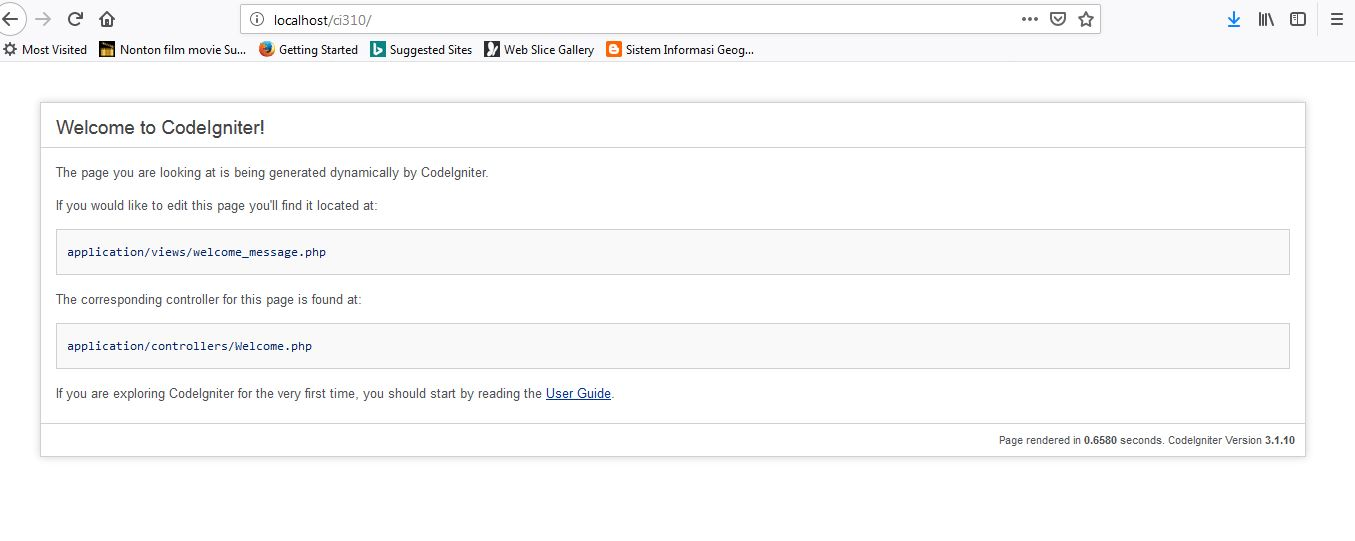
\includegraphics[width=1.0\textwidth]{figures/instalasi.JPG}}
\caption{Halaman Welcome dari CodeIgniter}
\label{Gambar 1}
\end{figure}

\section {Mengenal Pola Desain MVC}
\textit{Model,View,Controller} atau dengan singkatan \textit {MVC} adalah nama dari suatu metodologi atau pola desain \textit {design pattern} yang digunakan untuk merelasikan data dan \textit{user-interface} aplikasi secara efisien. pola awal MVC digunakan untuk rancang-bangun aplikasi desktop, khususnya untuk aplikasi-aplikasi yang dikembangkan menggunakan C++, Java,dan Smaltalk.
Dalam Pola MVC, komponen aplikasi dibagi menjadi tiga bagian yaitu :
\begin{enumerate}
\item \textit{Model} yang mempresentasikan struktur data.
\item \textit{View} yang merupakan repsentasi keluaran\textit{(output)}dari suatu model.
\item \textit{Controller} Komponen yang bertugas mengambil masukan \textit{(model dan view)}
\end{enumerate}
Secara umum, pola MVC dapat digambarkan sebagai berikut :
\begin{figure}[ht]
\center{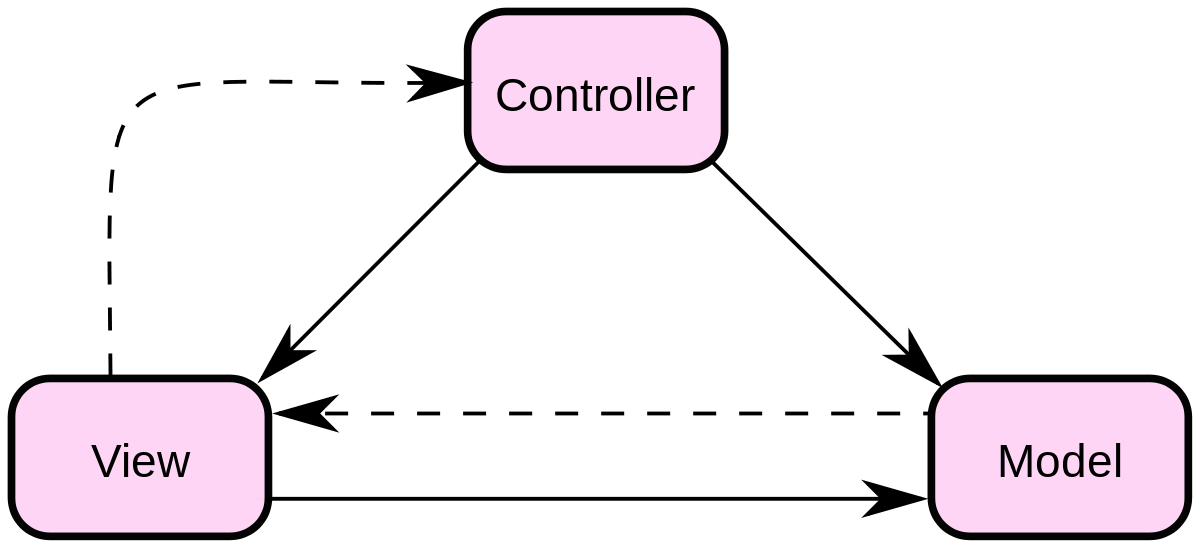
\includegraphics[width=1.0\textwidth]{figures/MVC.PNG}}
\caption{Arsitektur MVC}
\label{Gambar 2}
\end{figure}

\section{Struktur Direktori CodeIgner}
Dalam paket distribusinya, \textit{framework} CodeIgniter memiliki tiga direktori, yaitu :
\begin{enumerate}
\item application
\item system
\item user\_guide
\end{enumerate}

\subsection {Direktori application}
Direktori application adalah direktori yang digunakan untuk menempatkan file dari aplikasi yang akan kita buat. kita perlu menempatkan daftar \textit{model,controller,view} yang dibuat didalam direktori ini.
Penempatan file kedalam direktori appliaction harus diklarifikasikan sesuai ketentuan yang sudah ditetapkan oleh CodeIgniter. berikut dibawah ini adalah daftar sub-direktori dan penjelasan-penjelasnnya yang terdapat didalam direktori application
\begin{enumerate}
\item cache berguna untuk menyimpan halaman-halaman yang telah dibuku sebelumnya dan disembunyikan \textit{cached)}
\item config, berisi daftar file konfigurasi yang akan digunakan oleh aplikasi yang kita kembangkan
\item controllers, berisi daftar \textit{file controller}
\item core, digunakan untuk menempatkan daftar file kelas induk atau kelas dasar yang nantinya akan digunakan oleh aplikasi.
\item helpers, digunakan untuk menempatkan daftar file helper(pustaka dalam bentuk fungsi) yang didefenisikan sendiri.
\item hooks,digunakan untuk menyimpan file pendukung aplikasi
\item language, dalam direktori ini kita dapat mendefinisikan konstanta tertentu dalam bahasa yang diinginkan.
\item libraries, berisi file library (pustaka dalam bentuk kelas) yang kita definisikan sendiri.
\item logs, digunakan oleh CodeIgniter untuk menyimpan \textit{file log} (catatan) yang secara otomatis akan ditulis ketika terjadi kesalahan
\item models, berisi daftar \textit{model} yang kita perlukan oleh aplikasi.
\item third\_party, digunakan untuk menyimpan \textit{plugin} yang dikembangkan oleh pihak ketiga.
\item views, berisi daftar file \textit{view} yang diperlukan oleh aplikasi.
\end{enumerate}

